\documentclass[12pt,a4paper]{report}
\usepackage{amsmath,amsthm,amssymb}
\usepackage[utf8]{inputenc}
\usepackage[russian]{babel}
\usepackage[T2A]{fontenc}

\usepackage{mathtext}
\usepackage{graphicx}

\usepackage{cmap}


\DeclareMathSizes{12}{14}{10}{8}

\usepackage[left=30mm, right=15mm, top=20mm, bottom=20mm]{geometry}
\usepackage{indentfirst}
\usepackage{setspace}
\usepackage{multirow,makecell,array}
\usepackage{cite} 
\usepackage{enumerate}
\hyphenpenalty=10000 

%\usepackage{float}
\usepackage{floatrow}
\usepackage{calc}

\makeatletter
\bibliographystyle{utf8gost705u}
\usepackage{titlesec}
\usepackage[usenames]{color}
\usepackage{colortbl}
\setcounter{secnumdepth}{5} 
\usepackage{tocloft} 

\renewcommand{\tiny}{\fontsize{7}{8.4pt}\selectfont}
\renewcommand{\scriptsize}{\fontsize{9}{11pt}\selectfont}
\renewcommand{\footnotesize}{\fontsize{11}{13.6pt}\selectfont}
\renewcommand{\small}{\fontsize{12}{14.5pt}\selectfont}
\renewcommand{\normalsize}{\fontsize{14}{18pt}\selectfont}
\renewcommand{\large}{\fontsize{17}{20pt}\selectfont}
\renewcommand{\Large}{\fontsize{20}{25pt}\selectfont}

\usepackage{hyperref}
\providecommand{\phantomsection}{}


\newcommand{\ket}[1]{\left|#1\right\rangle}
\newcommand{\bra}[1]{\left\langle #1\right|}

\newcommand{\NL}[2]{#1_{\mbox{\tiny #2}}}

\newcommand{\VSD}{\NL{V}{SD}}
\newcommand{\VG}{\NL{V}{G}}
\newcommand{\kBT}{k_{\mbox{\tiny B}}T}
\newcommand{\sgn}{\mbox{sgn}}

\newcommand{\Cis}[1]{C^{\mbox{\tiny о}}_{#1}}
\newcommand{\hCis}{\hat{C}^{\mbox{\tiny о}}}
\newcommand{\Cel}[1]{C^{\mbox{\tiny э}}_{#1}}
\newcommand{\hCel}{\hat{C}^{\mbox{\tiny э}}}
\newcommand{\Cisel}[1]{C^{\mbox{\tiny о-э}}_{#1}}
\newcommand{\hCisel}{\hat{C}^{\mbox{\tiny о-э}}}

\newcommand{\qis}{q^{\mbox{\tiny о}}}
\newcommand{\qel}{q^{\mbox{\tiny э}}}
\newcommand{\nis}{n^{\mbox{\tiny о}}}
\newcommand{\nel}{n^{\mbox{\tiny э}}}
\newcommand{\phiis}{\phi^{\mbox{\tiny о}}}
\newcommand{\phiel}{\phi^{\mbox{\tiny э}}}

\DeclareFloatSeparators{mysep}{\hspace{1cm}}%какая-то штука для картинок в ряд, вроде расстояние между плавающими объектами
\DeclareFloatSeparators{mysep2}{\hspace{2cm}}
\begin{document}

% настройка отступов
\setlength{\parindent}{1.25cm} 
% убираем висячие строки  и подобное безобразие
\sloppy   
% Запрещаем разрыв страницы после первой строки абзаца
\clubpenalty=10000		
% Запрещаем разрыв страницы перед последней строкой абзаца
\widowpenalty=10000		

% Полуторный интервал
\onehalfspacing  
%%%%%%%%%%%%%%%%%%%%%%%%%%%%%%%%%%%%%%%%%%%%%%%%%%%%%%%%
%                    Титульный лист                    %
%%%%%%%%%%%%%%%%%%%%%%%%%%%%%%%%%%%%%%%%%%%%%%%%%%%%%%%%
\thispagestyle{empty}
\begin{titlepage}
\begin{center}
ФЕДЕРАЛЬНОЕ ГОСУДАРСТВЕННОЕ БЮДЖЕТНОЕ ОБРАЗОВАТЕЛЬНОЕ
УЧРЕЖДЕНИЕ ВЫСШЕГО ОБРАЗОВАНИЯ \\
«МОСКОВСКИЙ ГОСУДАРСТВЕННЫЙ УНИВЕРСИТЕТ\\
имени М.В.ЛОМОНОСОВА»
\vspace{1cm}

ФИЗИЧЕСКИЙ ФАКУЛЬТЕТ\\
\vspace{1cm}
КАФЕДРА ФИЗИКИ ПОЛУПРОВОДНИКОВ И КРИОЭЛЕКТРОНИКИ\\

\vspace{1cm}


\vspace{1cm}

\textbf{<<ИССЛЕДОВАНИЕ ТРАНСПОРТНЫХ ХАРАКТЕРИСТИК ОДНОЭЛЕКТРОННОГО ОДНОАТОМНОГО ТРАНЗИСТОРА>>}


\end{center}


\begin{flushright}
\vspace{1cm}

Выполнил студент \\
416 группы:\\

Назаров Степан Сергеевич \\

\underline{\hspace{3cm}}\\

\vspace{1cm}

Научный руководитель:\\
доцент, к.ф.\--м.н. Шорохов В.В. \\
\underline{\hspace{3cm}}\\
 
\end{flushright}

\vspace{1cm}
\begin{flushleft}

\vspace{1cm}
\end{flushleft}
\begin{center}
\vspace{1cm}
\small МОСКВА \\ \number\year\normalsize
\end{center}
\end{titlepage}



%%%%%%%%%%%%%%%%%%%%%%%%%%%%%%%%%%%%%%%%%%%%%%%%%%%%%%%%
%                      Оглавление                      %
%%%%%%%%%%%%%%%%%%%%%%%%%%%%%%%%%%%%%%%%%%%%%%%%%%%%%%%%
\setcounter{page}{2}
\tableofcontents

\section*{Мотивация}
\addcontentsline{toc}{section}{Мотивация}

Первые работы, сообщающие о реализации одноэлектронных устройств появились более 30 лет назад \cite{Likharev}. Одноэлектроника нашла применения в самых разных сферах:  термометрия\cite{Thermo}, память\cite{memory}, сенсоры\cite{sensor}.

Развитие технологических процессов в области изготовления полупроводниковых микросхем, привело к увеличению разрешающей способности, что позволяет уменьшить характерные размеры островков в устройствах. В наши дни на передовой находятся устройства с одиночными молекулами или атомами в роли зарядового центра \cite{SASET_EXP_OUR, SMSET, SASET_TOP}. 

Нельзя не упомянуть резервуарные вычислительные нейросети, первые шаги к созданиям которых уже были проделаны в работе \cite{neuro}. Сами авторы считают, что кластер наночастиц золота можно рассматривать, как набор туннельно связанных одноатомных одноэлектронных транзисторов. 

Уже были проведены теоретические работы по созданию обобщённых алгоритмов расчёта обычных одноэлектронных устройств \cite{Dobr}, где в роли зарядовых центров выступают металлические островки. Однако, с точки зрения практических применений (создание сенсоров, логических элементов) больший интерес проявляется к элементам из одиночных атомов и молекул. А значит, разработка универсальных методик расчёта для структур с дискретной энергетической структурой существенно расширит возможности на стадии проектирования подобного рода устройств.

\section*{Цель работы}

Целью данной бакалаврской работы является создание универсального алгоритма расчёта структур с атомной функциональной структурой, анализ и моделирование систем с такими структурами в роли ключевых элементов и применение данного алгоритма для объяснения наблюдаемых в эксперименте характеристик одноатомных одноэлектронных устройств.

\section*{Модель}
\addcontentsline{toc}{section}{Модель}

Классическая (ортодоксальная)\cite{Likharev} теория одноэлектроники при рассмотрении одноатомных одноэлектронных транзисторов  неприменима, ввиду дискретности энергетического спектра атома, как зарядового центра, и конечного числа зарядовых состояний. Соответственно, для расчёта характеристик таких устройств необходимо составление отдельной физической модели явления и её расчёт.

Необходимо смоделировать работу  одноатомного одноэлектронного транзистора. Типичное его устройство представлено на рис.\ref{fig:SASET}. Этот транзистор исследовался в работе \cite{patriot}. Кремниевые электроды на подложке из оксида кремния. Между электродами находится атом фосфора. 
\begin{figure}[h]
	\center{\includegraphics[scale=0.3]{patriot.png}}
	\caption{Одноатомный одноэлектронный транзистор}
	\label{fig:SASET}
\end{figure}
Электроды представим как три относительно больших проводящих сферы. Примесный атом отождествим с двумя концентрическими проводящими сферами. Две последних отвечают за представление электронных оболочек атома, по сути энергетических уровней. Можно взять и больше, но мы ограничимся двумя, для простоты изложения. Все геометрические размеры представлены на рис. \ref{fig:SASET model}.
\begin{figure}[h]
	\center{\includegraphics[scale=0.35]{SASET model}}
	\caption{Модель одноатомного одноэлектронного транзистора}
	\label{fig:SASET model}
\end{figure}
Каждая сфера из набора концентрических будет соответствовать отдельной оболочке и отдельному энергетическому уровню. Для наглядности и простоты вычислений пока ограничимся двумя. Мы так же пока не принимаем во внимание различие в формах атомных орбиталей в зависимости от их типа($s,p,d,f$). 

Так-же будем считать, что электроны могут туннелировать только со сфер Исток, Сток на сферы атома и в обратную сторону. Т.е. туннельного тока на Затвор нет.

Исток, Сток и Затвор поддерживаем при постоянном напряжении, то есть подаём на указанные сферы потенциалы $\varphi_s, \varphi_d, \varphi_g$ соответственно.

Нам так же потребуются значения энергии Ферми $\varepsilon_F$ для электродов и уровней атома $\mu_1, \mu_2$. Последние стоит отсчитывать от дна зоны проводимости для электрода.

Оканчивая постановку задачи, необходимо найти значение силы тока электронов с Истока на Сток, при заданных потенциалах на электродах $\varphi_s, \varphi_d, \varphi_g$. А для получения диаграмм стабильности, найти ток в каждой точке некоторого диапазона изменения потенциалов.
\section*{Изменение свободной энергии системы}
\addcontentsline{toc}{section}{Изменение свободной энергии системы}

Введём векторы зарядов и векторы потенциалов на рассматриваемых телах.
\begin{equation}
\vec{q} =  \left(
  \begin{array}{c}
    q_s\\
    q_d\\
    q_g\\
    q_1\\
    q_2\\
  \end{array}
  \right) = \left(
  \begin{array}{c}
  \vec{q_e}\\
  \vec{q_d}\\
  \end{array}
  \right)
  , 
  \vec{\varphi} = \left(
  \begin{array}{c}
  \varphi_s\\
  \varphi_d\\
  \varphi_g\\
  \varphi_1\\
  \varphi_2\\
  \end{array}
  \right) = \left(
  \begin{array}{c}
  \vec{\varphi_e}\\
  \vec{\varphi_d}\\
  \end{array}
  \right)
\end{equation}

Изменение энергии мы будем рассматривать за один акт туннелирования. Введём в рассмотрение начальные $\vec{\varphi}_{\mbox{i}}, \vec{q}_{\mbox{i}}$ и конечные $\vec{\varphi}_{\mbox{f}}, \vec{q}_{\mbox{f}}$ значения этих векторов. $\vec{q_e}, \vec{\varphi_e}$ — электродные компоненты векторов (от англ. electrode), так же являющиеся векторами, а $\vec{q_d}, \vec{\varphi_d}$ — атомные их компоненты (от англ. dopant). Для наглядности:
\begin{equation}
\vec{q_e} = \left(
\begin{array}{c}
q_s\\
q_d\\
q_g\\
\end{array}
\right),
\vec{\varphi_d} = \left(
\begin{array}{c}
\varphi_1\\
\varphi_2\\
\end{array}
\right)
\end{equation}

Изменение электростатической энергии запишем в виде
\begin{equation}
  dU = 
  \frac{\vec{\varphi_{f}^T}\vec{q}_{f}-\vec{\varphi_{i}^T}\vec{q}_{i}}{2}=
  \frac{(\vec{\varphi_{i}^T}+\vec{d\varphi^T})
  (\vec{q}_{i}+d\vec{q})
  -\vec{\varphi_{i}^T}\vec{q}_{i}}{2}
\end{equation}
Здесь $\vec{\varphi_{f}^T}$ — по сути строка, получающаяся транспонированием вектора. Заметим, поскольку электроды поддерживаются при постоянном потенциале, то 
вектор изменения потенциалов всех элементов 
\begin{equation}
  d\vec{\varphi}=
  \vec{\varphi}_{\mbox{f}}-\vec{\varphi}_{\mbox{i}}=
  \left(
  \begin{array}{c}
   \vec 0_e\\
   d\vec \varphi_d
  \end{array}
  \right)
\end{equation}
Вектор изменения зарядов всех элементов 
\begin{equation}
  d\vec{q}=
  \vec{q}_{\mbox{f}}-\vec{q}_{\mbox{i}}=
  \left(
  \begin{array}{c}
   d\vec q_{ind}+d\vec q_{tun}\\
   d\vec q_d
  \end{array}
  \right)=
  \left(
  \begin{array}{c}
   d\vec q_{ind}+ed\vec n_{tun}\\
   ed\vec n_d
  \end{array}
  \right),
\end{equation}
где $d\vec q_{ind}$ — вектор изменения индуцированных на электродах зарядах, $d\vec{n_{tun}}$ — вектор изменения заряда электродов вследствие туннелирования, $d\vec{n_d}$ — вектор изменения количества электронов на атомных уровнях.
Выражение для изменения свободной энергии можно переписать в следующем 
виде с учетом неизменности электрических потенциалов электродов
\begin{equation}
  dU = \frac{\vec{\varphi}^T_{\mbox{i}}d\vec{q}+
  \vec{q}^T_{\mbox{i}}d\vec{\varphi}+
  d\vec{q}^Td\vec{\varphi}}{2}=
  \frac{(\vec{q}^T_d+d\vec{q}^T_d)d\vec{\varphi}_d+
  \vec{\varphi}_d^Td\vec{q}_d+
  \vec{\varphi}_e^Td\vec{q}_{ind}}{2}
\end{equation}
Для нахождения $d\vec q_{ind}$, $\vec{\varphi}_d$ и 
$d\vec{\varphi}_d$ запишем систему уравнений
\begin{equation}\label{eq3}
  \left(
  \begin{array}{c}
   \vec q_{ind}\\
   \vec q_d
  \end{array}
  \right)=
  \left(
  \begin{array}{cc}
   \hat C_{ee} & \hat C_{ed}\\
   \hat C_{de} & \hat C_{dd}
  \end{array}
  \right)
  \left(
  \begin{array}{c}
   \vec \varphi_e\\
   \vec \varphi_d
  \end{array}
  \right)
\end{equation}
Обсуждение расчёта матрицы из последнего уравнения выходит за рамки нашего краткого повествования. Получим
\begin{equation}
  \begin{array}{l}
   \vec \varphi_d=\hat C^{-1}_{dd}
   (\vec{q}_d-\hat C_{de}\vec \varphi_e)\\
   \vec q_{ind}=(\hat C_{ee}-\hat C_{ed}\hat C^{-1}_{dd}\hat C_{de})\varphi_e+
   \hat C_{ed}\hat C^{-1}_{dd}\vec q_d.
  \end{array}
\end{equation}
На основе этих уравнений для $d\vec q_{ind}$ и 
$d\vec{\varphi}_d$ получаем:
\begin{equation}
  \begin{array}{l}
   d\vec \varphi_d=\hat C^{-1}_{dd}d\vec{q}_d\\
   d\vec q_{ind}=
   \hat C_{ed}\hat C^{-1}_{dd}d\vec q_d.
  \end{array}
\end{equation}
Получаем для изменения электростатической энергии
\begin{equation}
  dU = 
  \frac{(\vec{q}^T_d+d\vec{q}^T_d)\hat C^{-1}_{dd}d\vec{q}_d+
  (\vec{q}_d^T-\vec \varphi_e^T\hat C_{ed})\hat C^{-1}_{dd}d\vec{q}_d+
  \vec{\varphi}_e^T\hat C_{ed}\hat C^{-1}_{dd}d\vec q_d}{2}
\end{equation}
Окончательно изменения электростатической энергии:
\begin{equation}
  dU = \vec{q}^T_d\hat C^{-1}_{dd}d\vec{q}_d+
  \frac{d\vec{q}^T_d\hat C^{-1}_{dd}d\vec{q}_d}{2}=
  e^2\vec{n}^T_d\hat C^{-1}_{dd}d\vec{n}_d+
  \frac{e^2}{2}d\vec{n}^T_d\hat C^{-1}_{dd}d\vec{n}_d
\end{equation}
Изменение свободной энергии системы включает в себя работу источников
\begin{equation}\label{eq1}
 dF=dU + U=e^2\vec{n}^T_d\hat C^{-1}_{dd}d\vec{n}_d+
  \frac{e^2}{2}d\vec{n}^T_d\hat C^{-1}_{dd}d\vec{n}_d+
  e\vec \varphi_e^T(\hat C_{ed}\hat C^{-1}_{dd}d\vec{n}_d+d\vec{n}_{tun})
\end{equation}



\section*{Темп туннелирования}
\addcontentsline{toc}{section}{Темп туннелирования}
Распределение электронов по энергиям в электроде описывается
распределением Ферми-Дирака:
\begin{equation}
f(E)= \frac{1}{1+\exp(\frac{E-E_F}{kT})},
\end{equation}
где $E_F$ — энергия Ферми.
Ширина энергетических уровней в атоме описывается распределением Лоренца:
\begin{equation}
L(E)=\frac{1}{\pi}\frac{\gamma/2}{(E-E_0)^2+(\gamma/2)^2}
\end{equation}
Здесь $\gamma$ — полуширина энергетического уровня. $E_0$ — энергия уровня. Прозрачность туннельного барьера оценивается с помощью метода ВКБ:
\begin{equation}
\tau \approx \exp(-\frac{2}{\hbar}\sqrt{2m\Delta\mu}l),
\end{equation}
$\Delta\mu = \mu_d - \mu_e$ — изменение химического потенциала при туннелировании электрона с электрода на атом. $l$ есть расстояние между примесным атомом и электродом. Беря во внимание плотность электронных состояний $D$ на границе электрода, значение темпа туннелирования можно оценить следующим образом:
\begin{equation}\label{eq2}
\Gamma_{ed} = D\tau \int\limits_{-\infty}^{\infty}f(E)L(E + \Delta E) dE,
\end{equation} 
Причём $\Delta E = dF$, где $dF$ определяется из формулы (\ref{eq1}).
По физическому смыслу формула (\ref{eq2}) представляет собой формулу нахождения вероятности наступления двух независимых событий: наличие электрона с энергией $E$ в электроде <<попадание>> электрона после туннелирования в атомный уровень.
\begin{figure}[h]
	\center{\includegraphics[scale=0.7]{shock kontent}}
	\caption{Схематичное изображение зонной структуры}
	\label{fig:SASET model}
\end{figure}
Темп туннелирования с примесного атома на электрод даётся в свою очередь формулой:
\begin{equation}\label{eq4}
\Gamma_{de} = D\tau \int\limits_{-\infty}^{\infty}(1 - f(E + \Delta E))L(E) dE,
\end{equation}

\section*{Граф состояний}
\addcontentsline{toc}{section}{Граф состояний}
Пусть на островке между двумя электродами электрон может находиться лишь в двух энергетических состояниях. Согласно принципу Паули на каждом из уровней может находится максимум два электрона. Тогда система может находиться в одном из 16 состояний, причём возможны только строго определённые переходы между этими состояниями в процессе актов туннелирования. Эти состояния и разрешённые переходы между ними изображены на рис. \ref{fig:level-graph1}.

Пронумерованы они в двоичной системе счисления. Это очень удобно при численном моделировании данной системы, поскольку каждый разряд числа отвечает за наличие электрона с некоторым спином на данном энергетическом уровне.

\begin{figure}[h]
	\center{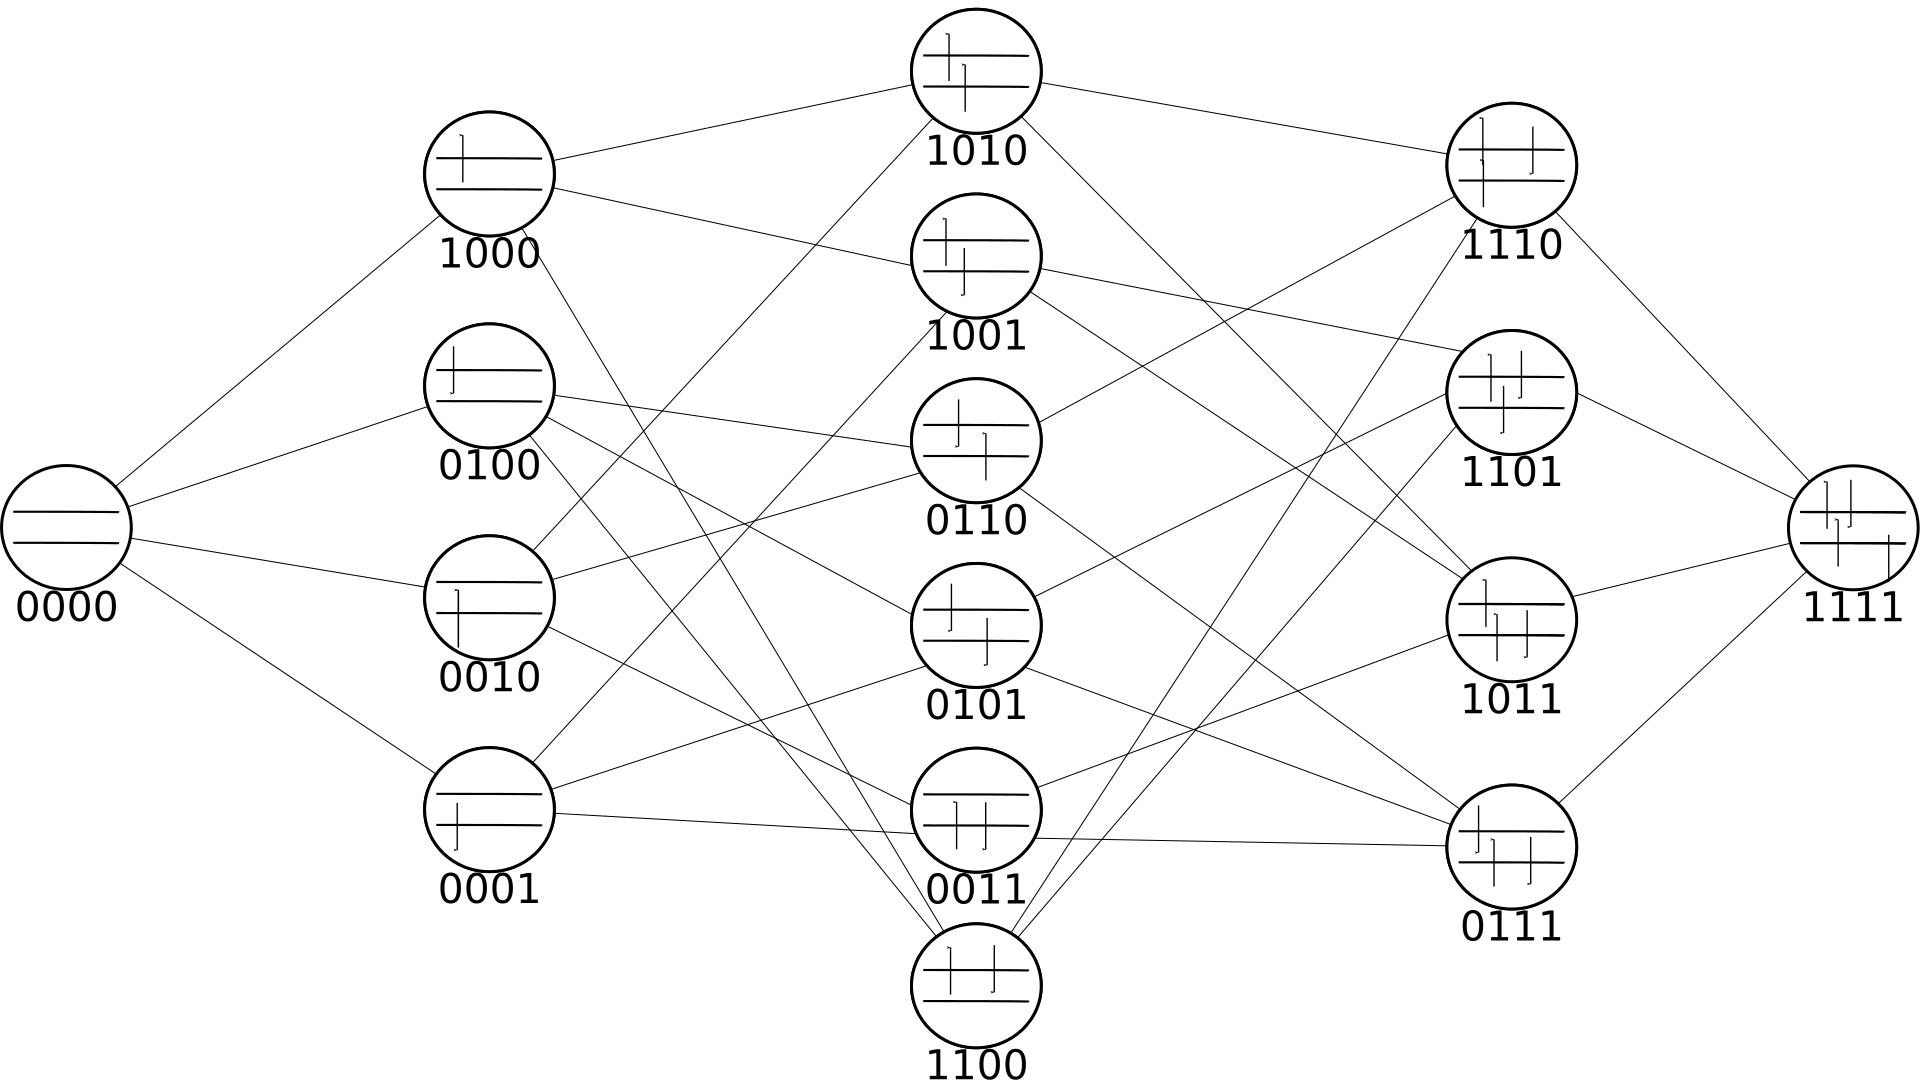
\includegraphics[scale=0.3]{level-graph.pdf}}
	\caption{Граф состояний двухуровневой системы}
	\label{fig:level-graph1}
\end{figure}

Таким образом можно сразу ввести эффективное, с точки зрения затрат вычислительных ресурсов, правило определения возможности перехода системы из одного зарядового состояния в другое: акт туннелирования возможен если побитовая запись номеров этих двух состояний отличается в одном и только в одном разряде. Для удобства дальнейшего повествования имеет смысл ввести логическую функцию $Graph(n, n')$, отвечающую правилу определения возможности перехода
\begin{equation}\label{rule}
Graph(n, n') =  \left\{
  \begin{array}{c}
    1\;\mbox{если переход $n \to n'$ возможен}\;,\\
    0\;\mbox{если переход $n \to n'$ невозможен}\;.
  \end{array}
  \right.
\end{equation}
$n$ и $n'$ здесь номера некоторых зарядовых состояний. 

В данной работе для расчёта тока использован метод решения системы кинетических уравнений \cite{kinetic}.

\section*{Обсуждение результатов}
\addcontentsline{toc}{section}{Обсуждение результатов}
Раз мы для простоты начали рассматривать систему с двумя уровнями, то результаты для начала представим для неё
\thisfloatsetup{floatrowsep=mysep}
\begin{figure}[h!]
\begin{floatrow}
   \ffigbox{\caption{Диаграмма стабильности системы с 2 уровнями}\label{fig:current_2lvl}}
           {\includegraphics[scale = 0.6]{current 2lvl}}
   \ffigbox{\caption{Среднее число электронов для системы с 2 уровнями}\label{fig:n_2lvl}}
           {\includegraphics[scale = 0.6]{n 2lvl}}  
\end{floatrow}    
\end{figure}
\thisfloatsetup{floatrowsep=mysep}
\begin{figure}[h!]
\begin{floatrow}
   \ffigbox{\caption{ВАХ для системы с двумя уровнями}\label{fig:VAH_2lvl}}
           {\includegraphics[scale = 0.5]{VAH 2lvl}}
   \ffigbox{\caption{Сигнальная характеристика для системы с 2 уровнями}\label{fig:signal}}
           {\includegraphics[scale = 0.5]{signal 2lvl}}  
\end{floatrow}    
\end{figure}
Как можно заметить, использованные в данной работе методы позволяют строить любые необходимые диаграммы. Однако, модель с двумя уровнями всё же является некоторой абстракцией, поведение которой на реальных системах заметить невозможно. Поэтому вниманию читателя представляется диаграмма стабильности для системы с 8 уровнями.
\begin{figure}[h]
	\center{\includegraphics[scale=0.5]{2}}
	\caption{Диаграмма стабильности для системы с 8 уровнями}
	\label{fig:8lvl}
\end{figure}
Так же стоит обратить внимание на экспериментальные диаграммы 
полученные в работе \cite{SASET_EXP_OUR}, изображённые на рис.\ref{fig:exp1} и рис.\ref{fig:exp2}.
\thisfloatsetup{floatrowsep=mysep}
\begin{figure}[h!]
\begin{floatrow}
   \ffigbox{\caption{Модуль тока из эксперимента}\label{fig:exp1}}
           {\includegraphics[scale = 0.35]{SASET exp our}}
   \ffigbox{\caption{Проводимость из эксперимента}\label{fig:exp2}}
           {\includegraphics[scale = 0.35]{SASET exp our der}}  
\end{floatrow}    
\end{figure}
Стоит заметить, что асимптотическое поведение экспериментальной диаграммы с рис.\ref{fig:exp1} очень хорошо прослеживается на диаграмме, полученной с помощью моделирования на рис.\ref{fig:8lvl}. А наклонные прямые на экспериментальной диаграмме проводимости на рис.\ref{fig:exp2} можно проследить на рассчитанной  диаграмме на рис.\ref{fig:current_2lvl}.

\section*{Итоги}
\addcontentsline{toc}{section}{Итоги}
Программа, моделирующая работу одноатомного транзистора была написана на языке C++, без использования сторонних библиотек. Данное ПО является полностью оригинальным. Преобразование данных расчёта в изображения производилось с помощью языка Python и библиотек NumPy, Matplotlib.

В заключении следует отметить несколько моментов, требующих доработки. Во-первых, приближение для значения $\tau$ является очень грубым и предполагает, что электрод и атом разделяет прямоугольный потенциальный барьер, что разумеется не так см. рис.\ref{fig:barrier}. 
\begin{figure}[h!]
	\center{\includegraphics[scale=0.3]{барьер}}
	\caption{Распределение потенциала в реальной системе и модели}
	\label{fig:barrier}
\end{figure}

Во-вторых, на вычисление интегралов в уравнениях (\ref{eq2}) и (\ref{eq4}) приходится огромная часть времени выполнения программы. Осмысленным является создание массива табличных значений данного интеграла и хранение его в виде отдельного файла для мгновенного доступа программы к значению интеграла.

В-третьих, необходимо применение алгоритмов работы с разреженными матрицами для решения системы кинетических уравнений, т.к. размер данной матрицы экспоненциально растёт с увеличением количества свободных мест для электронов на атомных оболочках, а матрица системы остаётся заполненной преимущественно нулями.
\renewcommand\bibname{Cписок литературы}
\addcontentsline{toc}{section}{Cписок литературы}
\begin{thebibliography}{99}

	\bibitem{Likharev}D.V. Averin and K.K. Likharev. Single electronics: A correlated transfer of single
electrons and cooper pairs in systems of small tunnel junctions. In B.L. ALTSHULER,
P.A. LEE, and R.A. WEBB, editors, Mesoscopic Phenomena in Solids, volume 30 of
Modern Problems in Condensed Matter Sciences, chapter 6, pages 173–271. Elsevier,
1991.
	\bibitem{Thermo} J. P. Pekola, J. K. Suoknuuti, J. P. Kauppinen, M. Weiss, P. v. d. Linden, and A. G. M.
Jansen. Coulomb blockade thermometry in the milli-kelvin temperature range in high
magnetic fields. Journal of Low Temperature Physics, 128(5):263–269, Sep 2002.
	\bibitem{memory} K. Nakazato, R. J. Blaikie, and H. Ahmed. Single-electron memory. Journal of Applied
Physics, 75(10):5123–5134, 1994.
	\bibitem{sensor} Knobel, R., Cleland, A. Nanometre-scale displacement sensing using a single electron transistor. Nature 424, 291–293 (2003).
	\bibitem{SASET_EXP_OUR} V. V. Shorokhov, D. E. Presnov, S. V. Amitonov, Yu. A. Pashkin, and V. A. Krupenin.Single-electron tunneling through an individual arsenic dopant in silicon
Nanoscale, 9:613–620, 2017.
	\bibitem{SMSET} Kubatkin, S., Danilov, A., Hjort, M. et al. Single-electron transistor of a single organic molecule with access to several redox states. Nature 425, 698–701 (2003).
	\bibitem{SASET_TOP} Fuechsle, M., Miwa, J., Mahapatra, S. et al. A single-atom transistor. Nature Nanotech 7, 242–246 (2012)
		\bibitem{neuro} Bose, S., Lawrence, C., Liu, Z. et al. Evolution of a designless nanoparticle network into reconfigurable Boolean logic. Nature Nanotech 10, 1048–1052 (2015).
	\bibitem{Dobr} D. M. Dobrynin, V. V. Shorokhov, and V. A. Krupenin. Correlated parallel electron
transport in double- and triple-island single-electron transistors. Journal of Physics: Conference Series, 1482:012027, mar 2020.
	\bibitem{patriot} Dagesyan, S.A., Shorokhov, V.V., Presnov, D.E., Soldatov, E.S., Trifonov, A.S., and Krupenin, V.A. Sequential reduction of the silicon single-electron transistor structure to atomic scale. Nanotechnology 28 (2017), 225304.
	\bibitem{kinetic} Alexander N. Korotkov. Coulomb blockade and digital single-electron devices, 1996.

\end{thebibliography}

\end{document}
